% !TeX encoding = UTF-8
% !TeX spellcheck = sk_SK
% !TeX TS-program = xelatex

\documentclass[a4paper,titlepage,12pt]{article}
\usepackage{geometry}
\usepackage[slovak]{babel}
\usepackage[table]{xcolor}
\usepackage{graphicx}
\usepackage{verbatim}
\usepackage{fancyhdr}
\usepackage{hyperref}
\usepackage{booktabs}
\usepackage{multirow}
\usepackage{tabularx}
\usepackage{caption}
\usepackage{amsmath}
\frenchspacing

\geometry{a4paper, left=3.00cm, right=2.50cm, top=3.50cm, bottom=2.75cm}
\renewcommand{\baselinestretch}{1.2}
\renewcommand{\arraystretch}{1.4}
\graphicspath{{figures/}}

\title{\textbf{Kreslenie elektrotechnických schém pomocou aplikácie QElektroTech}}
\author{}
\date{Posledná úprava \\ \today}

\hypersetup{
	pdfborder=0 0 0,
	colorlinks=false,
	linkcolor=blue,
	pdffitwindow=false,
	pdfstartview={FitB}
} 

\begin{document}
\maketitle
\tableofcontents
\newpage

\section{Nastavenie aplikácie QElektroTech}
Pred vytvorením projektu a samotným kreslením je potrebné venovať chvíľu času nastaveniam aplikácie QElektroTech. V nasledujúcich kapitolách sú uvedené nastavenia prostredia a nastavenia projektu.

\subsection{Nastavenie prostredia}
\begin{figure}[ht]
\centering
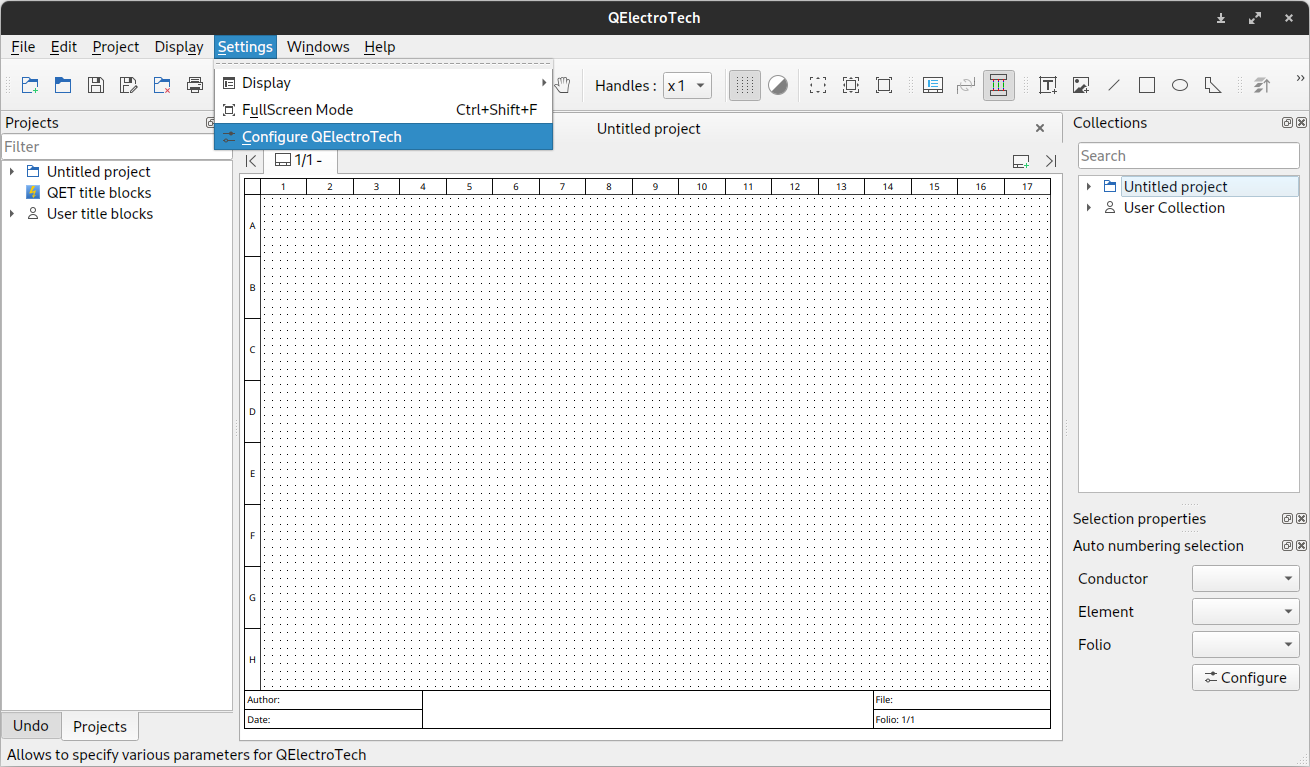
\includegraphics[width=0.75\textwidth]{settings-1.png}
\caption{Nastavenia aplikácie}
\label{Fig:nastavenia-aplikacie}
\end{figure}

\begin{figure}[ht]
\centering
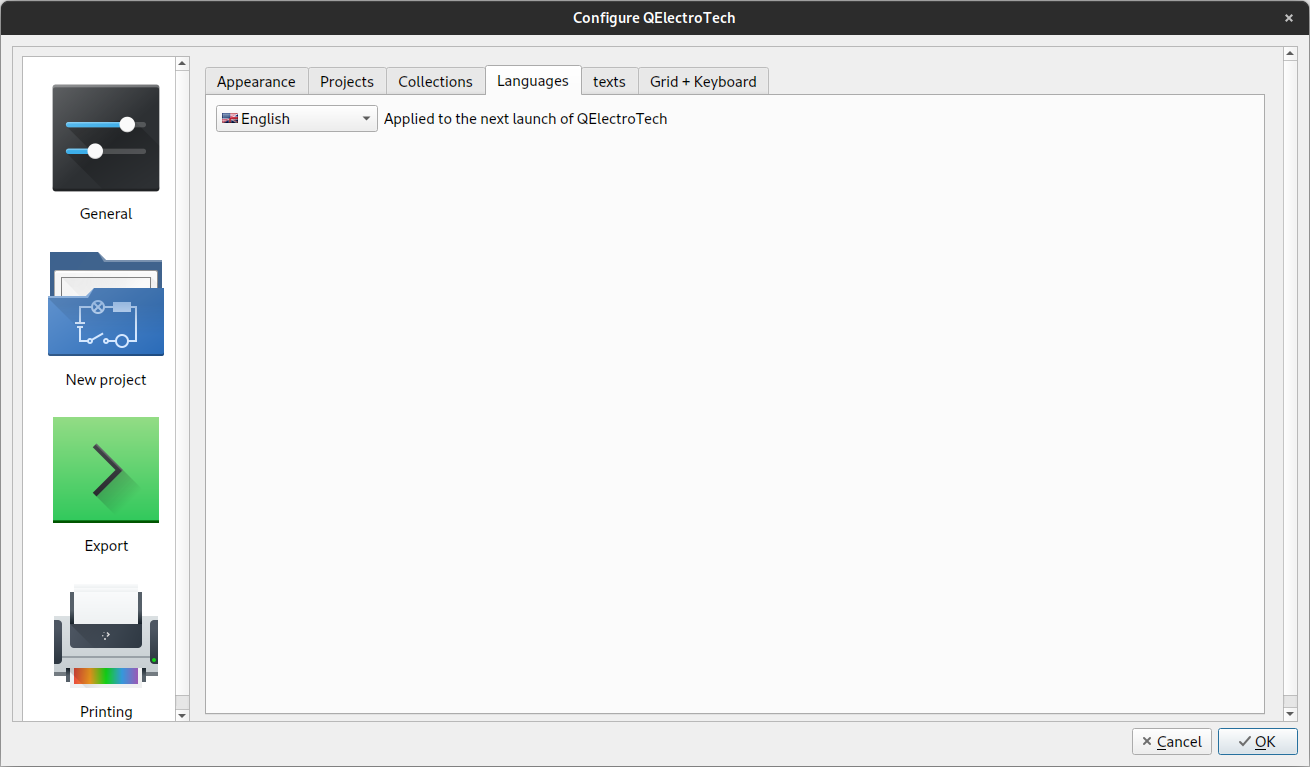
\includegraphics[width=0.75\textwidth]{settings-2.png}
\caption{Nastavenie jazyka}
\label{Fig:nastavenie-jazyka}
\end{figure}

\begin{figure}[ht]
\centering
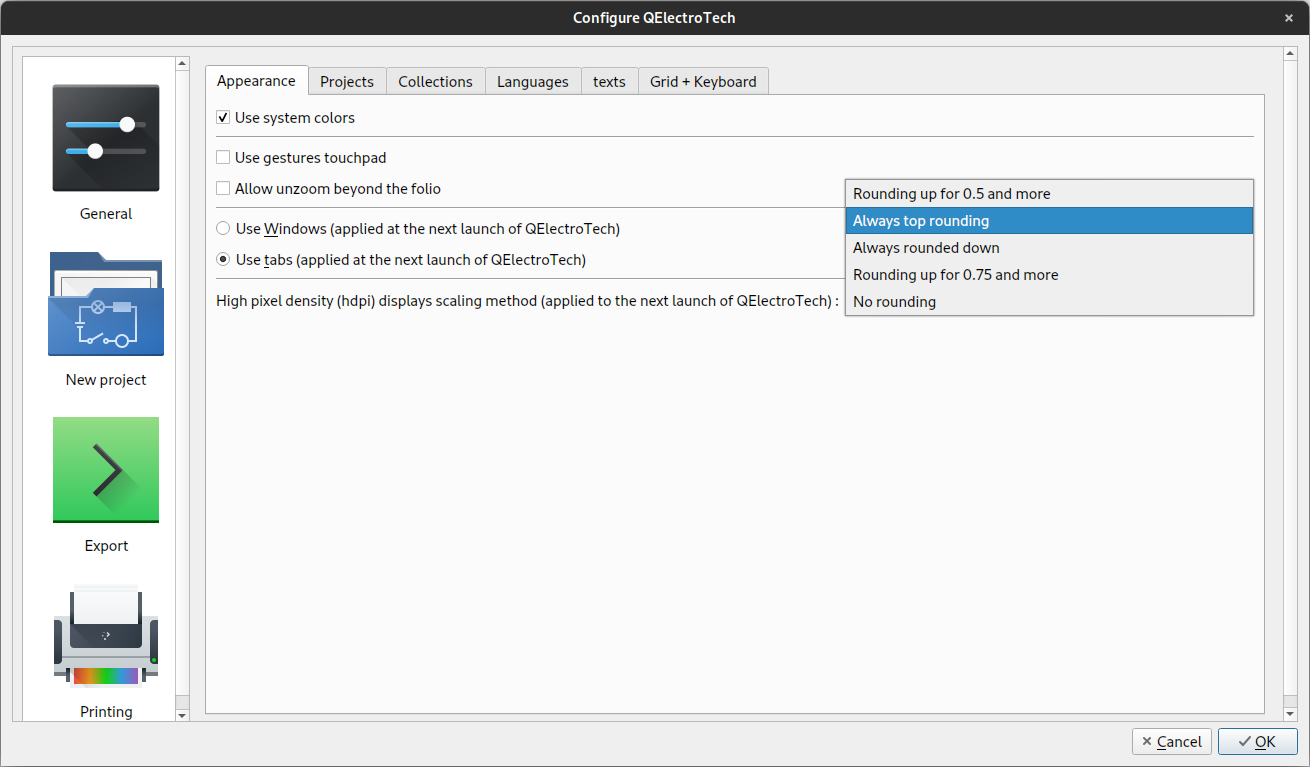
\includegraphics[width=0.75\textwidth]{settings-3.png}
\caption{Vyhladzovanie pre HDPI displeje}
\label{Fig:nastavenia-aplikacie}
\end{figure}

\subsection{Nastavenie projektu}

\end{document}
